% ============================================================
%  Příprava na maturitu – Elektrotechnika
%  Okruh 7: Točivé elektrické stroje
% ============================================================

\documentclass[a4paper,10pt]{article}

\usepackage[T1]{fontenc}
\usepackage[utf8]{inputenc}
\usepackage[left=2.0cm, right=1.8cm, top=1.8cm, bottom=1.8cm]{geometry}
\usepackage{parskip}
\usepackage{xcolor}
\usepackage{tabularx}
\usepackage{booktabs}
\usepackage{tikz}
\usepackage{mdframed}
\usepackage{amsmath}
\usepackage{enumitem}
\usepackage{circuitikz}

\usetikzlibrary{arrows.meta, positioning, decorations.pathmorphing, shapes.geometric, calc}

% --- Barvy ---
\definecolor{accent}{HTML}{1A3A5C}
\definecolor{lightblue}{HTML}{EAF2F8}
\definecolor{lightyellow}{HTML}{FDFBE4}
\definecolor{lightgreen}{HTML}{EAF7EA}
\definecolor{lightred}{HTML}{FDE8E8}
\definecolor{lightgray}{HTML}{F4F4F4}

% --- Boxy ---
\newmdenv[backgroundcolor=lightblue,linecolor=accent!40,roundcorner=4pt,
  innertopmargin=6pt,innerbottommargin=6pt,innerleftmargin=8pt,innerrightmargin=8pt]{pojmybox}
\newmdenv[backgroundcolor=lightyellow,linecolor=accent!30,roundcorner=4pt,
  innertopmargin=6pt,innerbottommargin=6pt,innerleftmargin=8pt,innerrightmargin=8pt]{vysvetlenibox}
\newmdenv[backgroundcolor=lightgreen,linecolor=accent!40,roundcorner=4pt,
  innertopmargin=6pt,innerbottommargin=6pt,innerleftmargin=8pt,innerrightmargin=8pt]{vzorcebox}
\newmdenv[backgroundcolor=lightred,linecolor=accent!30,roundcorner=4pt,
  innertopmargin=6pt,innerbottommargin=6pt,innerleftmargin=8pt,innerrightmargin=8pt]{durazbox}

\setlist[itemize]{noitemsep, leftmargin=1.4em, topsep=2pt}
\setlist[enumerate]{noitemsep, leftmargin=1.4em, topsep=2pt}

% --- Zkratka pro jednotky ---
\newcommand{\jednotka}[1]{\,[\mathrm{#1}]}

\begin{document}

% ============================================================
\section*{\large Okruh 7 – Točivé elektrické stroje}

\begin{pojmybox}
\textbf{Klíčové pojmy:}
stator, rotor, točivé magnetické pole, synchronní otáčky, asynchronní motor (kotva nakrátko / kroužková), skluz, synchronní stroj (alternátor), stejnosměrný motor, komutátor, dynamo, univerzální motorek
\end{pojmybox}

\begin{vysvetlenibox}

% ================================================================
\subsection*{1. Vznik točivého magnetického pole}

Většina střídavých motorů využívá k pohybu \textbf{točivé magnetické pole}. Vznikne tak, že na stator umístíme tři cívky prostorově posunuté o $120^\circ$ a připojíme je na trojfázové napětí (které je časově posunuté o $120^\circ$). Součtem jejich proměnných magnetických polí vznikne výsledné pole, které plynule rotuje.

\begin{vzorcebox}
\textbf{Synchronní otáčky točivého pole:}
\[
n_s = \frac{60 \cdot f}{p} \jednotka{ot/min}
\]
kde $f$ = frekvence sítě [Hz] (v ČR 50 Hz), $p$ = počet \textbf{pólových dvojic}.
\end{vzorcebox}
\textit{Příklad:} Pro $f = 50\,\mathrm{Hz}$ a $p = 1$ (dvoupólový stroj) jsou synchronní otáčky $3000\,\mathrm{ot/min}$. Pro $p = 2$ jsou $1500\,\mathrm{ot/min}$.

% ================================================================
\subsection*{2. Asynchronní motor (ASM)}

Nejpoužívanější průmyslový motor. Nemá žádné kartáče (v základní verzi), je levný a bezúdržbový.

\textbf{Princip:} Stator vytvoří točivé magnetické pole. To protíná vodiče rotoru a indukuje v nich napětí (Faradayův zákon). Protože je rotor spojen nakrátko, začnou v něm téct velké proudy. Tyto proudy vytvoří vlastní magnetické pole, které se snaží zachytit točivé pole statoru. Vzniká točivý moment.

\begin{durazbox}
\textbf{Proč se jmenuje asynchronní?} Rotor se \textbf{nikdy} nemůže točit synchronními otáčkami ($n_s$). Kdyby se točil stejně rychle jako pole, pole by neprotínalo vodiče rotoru $\implies$ neindukovalo by se napětí $\implies$ nebyl by proud $\implies$ nebyl by moment. Rotor se tedy vždy točí o něco pomaleji.
\end{durazbox}

\begin{vzorcebox}
\textbf{Skluz ($s$):} Relativní zpoždění rotoru za točivým polem statoru.
\[
s = \frac{n_s - n}{n_s} \cdot 100 \jednotka{\%}
\]
kde $n_s$ = otáčky magnetického pole, $n$ = skutečné otáčky rotoru. Běžně je $s = 2 \text{ až } 5\,\%$.
\end{vzorcebox}

\textbf{Konstrukce rotoru:}
\begin{itemize}
  \item \textbf{Kotva nakrátko (klec):} Hliníkové tyče zalité v drážkách rotoru, na koncích spojené kruhy. Jednoduchá.
  \item \textbf{Kroužkový rotor:} Vinutý rotor vyvedený přes sběrací kroužky a kartáče na svorkovnici. Umožňuje připojit externí odpory do rotoru pro \textbf{plynulý rozběh} s velkým momentem (omezení obrovského záběrového proudu).
\end{itemize}

\begin{center}
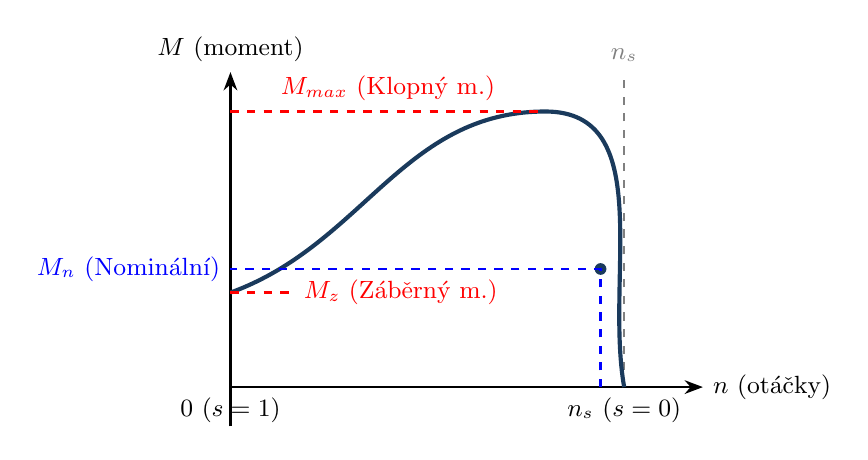
\begin{tikzpicture}[>=Stealth, font=\small, thick]
  % Momentová charakteristika ASM
  \draw[->] (0,0) -- (6,0) node[right] {$n$ (otáčky)};
  \draw[->] (0,-0.5) -- (0,4) node[above] {$M$ (moment)};
  
  % Osa synchronních otáček
  \draw[dashed, gray] (5,0) -- (5,4) node[above] {$n_s$};
  \node[below] at (5,0) {$n_s$ ($s=0$)};
  \node[below] at (0,0) {$0$ ($s=1$)};
  
  % Křivka
  \draw[accent, line width=1.5pt] (0, 1.2) to[out=20, in=180] (4, 3.5) to[out=0, in=100] (5, 0);
  
  % Popisky
  \draw[dashed, red] (0,1.2) -- (0.8,1.2) node[right, red] {$M_z$ (Záběrný m.)};
  \draw[dashed, red] (0,3.5) -- (4,3.5) node[midway, above, red] {$M_{max}$ (Klopný m.)};
  \node[circle, fill=accent, inner sep=1.5pt] at (4.7, 1.5) {};
  \draw[dashed, blue] (4.7,0) -- (4.7,1.5) -- (0,1.5) node[left, blue] {$M_n$ (Nominální)};
\end{tikzpicture}
\end{center}

% ================================================================
\subsection*{3. Synchronní stroje}

Stator je stejný jako u ASM (3f vinutí).
Rotor je ale napájen \textbf{stejnosměrným proudem} přes kroužky (tvoří elektromagnet) nebo je tvořen permanentními magnety.

\textbf{Princip:} Magnet rotoru se "uzamkne" do točivého magnetického pole statoru a točí se \textbf{zcela synchronně} s ním ($n = n_s$, skluz $s = 0$).

\textbf{Použití:}
\begin{itemize}
  \item \textbf{Alternátor (generátor):} Základní prvek v elektrárnách (výroba 3f proudu). Parní turbína točí rotorem (elektromagnetem) a ten ve statoru indukuje střídavé napětí (\textit{navazuje na Okruh 8}).
  \item \textbf{Motor:} Většinou se sám nerozběhne (musí se roztočit pomocí frekvenčního měniče nebo pomocného ASM). Používá se pro obrovské výkony (dmychadla, čerpadla) nebo naopak jako precizní servomotory.
\end{itemize}

% ================================================================
\subsection*{4. Stejnosměrné stroje a Komutátor}

Pracují se stejnosměrným proudem (DC). Obrovskou výhodou DC motorů je velmi jednoduchá a přesná regulace otáček.

\textbf{Komutátor:} Mechanický střídač/usměrňovač na rotoru. Je to válec z měděných lamel oddělených slídou. Přiléhají na něj uhlíkové \textbf{kartáče}. Komutátor při otáčení přepíná směr proudu v cívkách rotoru tak, aby točivý moment působil stále jedním směrem.

\begin{center}
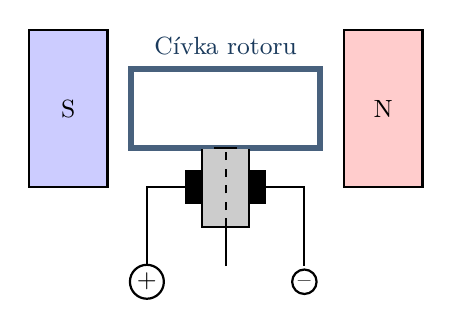
\begin{tikzpicture}[>=Stealth, font=\small, thick]
  % Stator poles
  \draw[fill=blue!20] (-2.5,-1) rectangle (-1.5,1);
  \node at (-2,0) {S};
  \draw[fill=red!20] (1.5,-1) rectangle (2.5,1);
  \node at (2,0) {N};
  
  % Rotor (kotva) - simplified
  \draw[accent!80, line width=2pt] (-1.2,-0.5) rectangle (1.2,0.5);
  \node[accent] at (0,0.8) {Cívka rotoru};
  
  % Komutátor a osa
  \draw[fill=gray!40] (-0.3,-1.5) rectangle (0.3,-0.5);
  \draw[dashed] (0,-1.5) -- (0, -0.5); % rozdělení lamel
  \draw (0,-2) -- (0,-1.5); % Osa
  
  % Kartáče
  \draw[fill=black] (-0.5,-1.2) rectangle (-0.3,-0.8);
  \draw[fill=black] (0.3,-1.2) rectangle (0.5,-0.8);
  
  % Připojení zdroje
  \draw (-0.5,-1) -- (-1,-1) -- (-1,-2);
  \draw (0.5,-1) -- (1,-1) -- (1,-2);
  \node[circle, draw, inner sep=1pt] at (-1,-2.2) {+};
  \node[circle, draw, inner sep=1pt] at (1,-2.2) {--};
  
  % Vodiče k cívce rotoru
  \draw[accent!80, line width=1pt] (-0.15,-0.5) -- (-1.2, -0.5);
  \draw[accent!80, line width=1pt] (0.15,-0.5) -- (1.2, -0.5);
\end{tikzpicture}
\end{center}

\textbf{Rozdělení DC motorů (podle zapojení buzení statoru):}
\begin{itemize}
  \item \textbf{Sériový:} Stator zapojen do série s rotorem. Má \textbf{obrovský záběrný moment}, který se zvyšuje se zátěží. Při odlehčení má snahu se "roztrhnout" (otáčky letí do nekonečna). \textit{Použití: Trakce (vlaky, tramvaje), startéry aut.}
  \item \textbf{Derivační:} Stator paralelně k rotoru. Otáčky jsou téměř nezávislé na zátěži (tvrdá charakteristika).
\end{itemize}

% ================================================================
\subsection*{5. Univerzální motorek}

Je to v podstatě sériový stejnosměrný motor upravený (složením jádra z plechů, aby se omezily vířivé proudy) tak, aby fungoval i na střídavý proud (AC). 
Protože se směr proudu ve statoru i rotoru mění současně, točivý moment má stále stejný směr.
\textbf{Vlastnosti:} Obrovské otáčky (až 30 000 ot/min), velký výkon při malých rozměrech.
\textbf{Použití:} Ruční nářadí (vrtačky, flexy), domácí spotřebiče (vysavače, mixéry). Nevýhodou je hlučnost a opotřebení kartáčů.

% ================================================================
\subsection*{6. Shrnutí – přehled vzorců}

\begin{center}
\begin{tabularx}{0.97\linewidth}{@{} l l l @{}}
\toprule
\textbf{Veličina} & \textbf{Vzorec} & \textbf{Jednotka} \\
\midrule
Synchronní otáčky & $n_s = \dfrac{60 \cdot f}{p}$ & ot/min \\
Skluz ASM & $s = \dfrac{n_s - n}{n_s}$ & -- (nebo \%) \\
Úhlová rychlost rotoru & $\omega = \dfrac{2\pi \cdot n}{60}$ & rad/s \\
Točivý moment & $M = \dfrac{P}{\omega}$ & Nm (newtonmetr) \\
\bottomrule
\end{tabularx}
\end{center}

\end{vysvetlenibox}

\end{document}